\section{PIA (Periferal Interface Adapter)}

La \textbf{PIA (Periferal Interface adapter)} è un dispositivo di comunicazione parallela ad 8 bit. Tale architettura è un dispositivo hardware che si posiziona tra la periferica e il processore stesso. Essa è costituita architetturalmente da due tipologie diverse di porto, il porto A ed il porto B.[\ref{img:PIA}]
Tali porti hanno dei registri che sono direzionali, quindi possono assumere una sola funzione (tra entrata ed uscita), in base alla loro specifica impostazione e configurazione.
Prima di parlare di più porti ci concentriamo sulle comunicazioni a singolo porto; in generale le comunicazioni che avvengono tra due interfacce della PIA sono configurabili tramite i bit di configurazione del chipset. Nel nostro caso, la comunicazione che maggiormente utilizzeremo è quella dotata di handshacking, per cui si avrà una configuraizone ed un collegamento simile all'immagine [\ref{img:PIA-CON}].
Il dispositivo PIA simulato in ASIM è derivato da quello commerciale MC6821. Questo è dotato di sei registri a 8 bit, tra cui: due registri per il trasferimento dei dati da e verso la periferica (\textit{PRA} e \textit{PRB}); due registri di controllo/stato (\textit{CRA} e \textit{CRB}); infine due registri per il controllo della direzione dei dati (\textit{DRA} e \textit{DRB}). Questi registri sono accessibili mediante indirizzamento interno secondo la tabella \ref{Tab:reg_ind_1}:

\begin{table} [!h]
    \centering
    \begin{tabular}{|c|c|c|c|c|}
        \hline
        \multicolumn{5}{|c|}{\textbf{Indirizzamento interno}} \\ \hline
        \textbf{RS1} & \textbf{RS0} & \textbf{CRA2} & \textbf{CRB2} & \textbf{Registro selezionato}\\ \hline
        0       &0      &1      &X      &PRA    \\  \hline
        0       &0      &0      &X      &DRA    \\  \hline
        0       &1      &X      &X      &CRA    \\  \hline
        1       &0      &X      &1      &PRB    \\  \hline
        1       &0      &X      &0      &DRB    \\  \hline
        1       &1      &X      &X      &CRB    \\  \hline
    \end{tabular}
    \caption{Indirizzamento interno}
    \label{Tab:reg_ind_1}
\end{table}

Questi registri sono selezionabili dal processore mediante le linee RS1 ed RS0.
Nel dettaglio, i registri di contollo sono a 8 bit suddivisi come indicato in tabella \ref{Tab:control_registers}:

\begin{table}[!ht]
    \centering
    \renewcommand{\arraystretch}{1.5} % Aumenta l'altezza delle righe
    \setlength{\tabcolsep}{8pt} % Uniforma la distanza tra colonne
    \begin{tabular}{|c|c|c|c|c|c|c|c|c|}
        \hline
        \multirow{2}{*}{\textbf{CRA}} 
        & \textbf{7}  & \textbf{6}  & \textbf{5}  & \textbf{4}  & \textbf{3}  & \textbf{2}  & \textbf{1}  & \textbf{0}  \\ 
        \cline{2-9} 
        & \textit{IRQA1}  & \textit{IRQA2}  
        & \multicolumn{3}{c|}{\textit{controllo CA2}}  
        & \textit{Accesso DRA}  
        & \multicolumn{2}{c|}{\textit{controllo CA1}}  \\ 
        \hline
        \multirow{2}{*}{\textbf{CRB}}  
        & \textbf{7}  & \textbf{6}  & \textbf{5}  & \textbf{4}  & \textbf{3}  & \textbf{2}  & \textbf{1}  & \textbf{0}  \\ 
        \cline{2-9} 
        & \textit{IRQB1}  & \textit{IRQB2}  
        & \multicolumn{3}{c|}{\textit{controllo CB2}}  
        & \textit{Accesso DRB}  
        & \multicolumn{2}{c|}{\textit{controllo CB1}}  \\ 
        \hline
    \end{tabular}
    \caption{Control Registers}
    \label{Tab:control_registers}
\end{table}



Entrando nei dettagli del processo, bisognerà fare particolare attenzione ai seguenti registri:
\begin{itemize}
    \item \textbf{CA1,CB1}: Sono registri che possono assumere solo direzione di ingresso e solitamente vengono usati come "lettori" di segnali SYN o segnali ACK da parte dell'altro dispositivo;
    \item \textbf{CA2,CB2}: Sono i registri che possono essere configurati(sia di ingresso che di uscita), ed in generale, in base al protocollo che si vuole interpretare, vengono settati in una determinata modalità di funzionamento (dipendente dalla tipologia di protocollo che si vuole implementare);
    \item \textbf{Dato}: Il bus dati trasmette parallelamente i dati tra le due periferiche in base al protocollo di handshacking utilizzato. I bus dati sono unidirezionali ma la direzione è programmabile. 
\end{itemize}

\begin{figure}
    \centering
    % 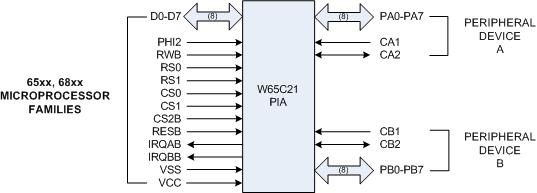
\includegraphics[width=0.45\textwidth]{img/PIA.png}
    % \hfill
    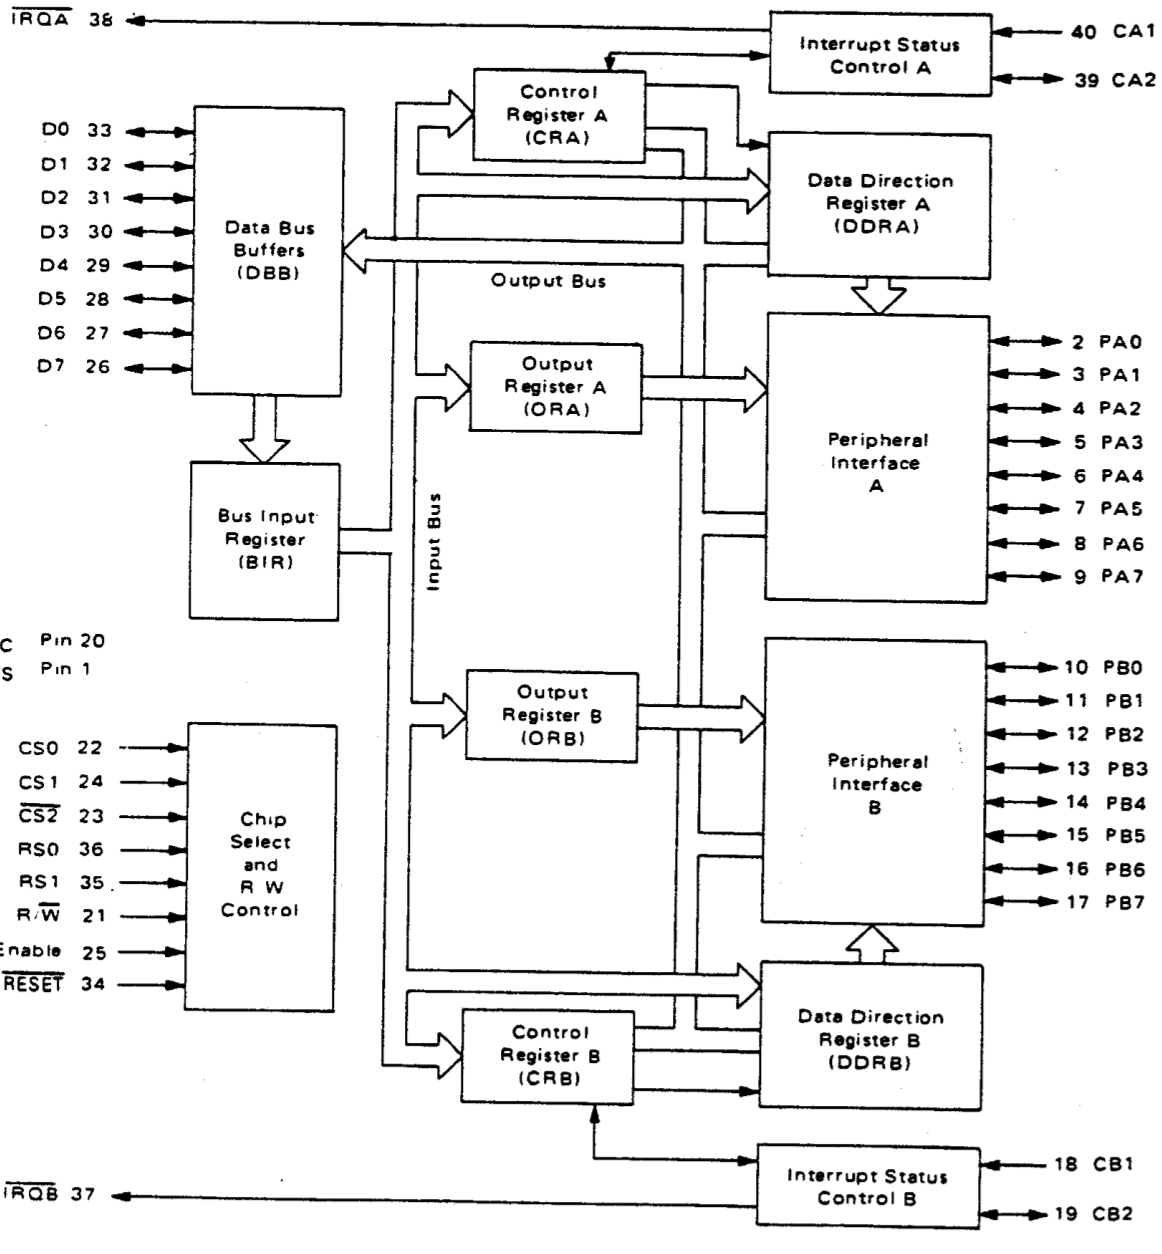
\includegraphics[width=0.75\textwidth]{img/PIA-SCHEME.jpg}
    \caption{Architettura base della PIA}\label{img:PIA}
\end{figure}

\begin{figure}
    \centering
    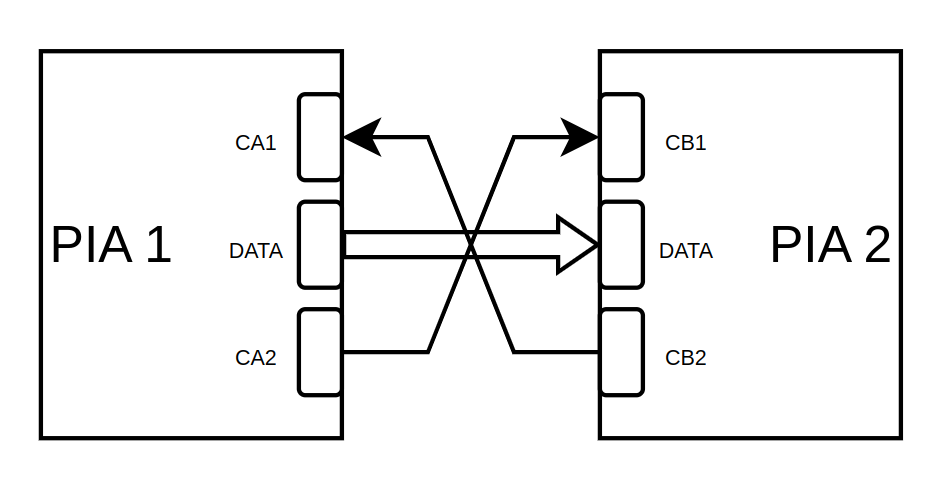
\includegraphics[width=0.65\textwidth]{img/PIA-CON.png}
    \caption{Collegamento tra due dispositivi tramite PIA}\label{img:PIA-CON}
\end{figure}

Per far si che le due architetture possano comunicare è quindi importante definire come si andranno a collegare e quindi la direzione e l'interpretazione che bisogna dare ai registri. Una possibile architettura di collegamento è quella visibile all'immagine [\ref{img:PIA-CON}].
Le linee D0-D7 sono di interfacciamento con il processore e sono bidirezionali in base alla natura dell'operazione richiesta (lettura o scrittura). 
Poiché la PIA ha due porti distinti, può essere collegata al processore con due linee di interruzioni differenti denominate \textbf{IRQA} (porto A) e \textbf{IRQB} (porto B).  

Una volta definita la tipologia di architettura si va a decidere come queste periferiche dovranno interagire tra loro (definizione del protocollo), per cui si va ad impostare uno specifico registro di configurazione che permetterà di impostare le seguenti opzioni:

\begin{itemize}
    \item \textbf{Interrupt o polling}: A che livello di priorità si andrà ad impostare l'interruzione della PIA;
    \item \textbf{Modalità di funzionamento}: se attuo l'handshacking o altre tipologie di protocolli;
    \item \textbf{Lettura o scrittura}: 

 
\end{itemize}
Una volta definita la struttura del registro di configurazione questo viene settato per impostare la PIA. 
Una volta impostato il modo di funzionamento si va a gestire il tutto. Qundi, se si è scelto un funzionamento tramite interrupt si avrà un certo tipo di comportamento, altrimenti se ne avrà un altro.

Il funzionamento generale della fase di \textbf{handshaking} tra due dispositivi PIA è gestita, per i nostri esempi, in un particolare modo.
Per fare chiarezza andremo a dividere la fase di ricezione dalla fase di trasmissione.
In fase di \textbf{trasmissione} le operazioni che si vanno ad effettuare sonno le seguenti:
\begin{itemize}
    \item \textbf{Inserimento del dato}: La periferica posiziona il dato sul bus dati collegato in maniera diretta con la PIA. Una volta effettuato l'inserimento, la periferica tramite la linea CA1 invia un segnale di \textit{dato pronto} alla PIA, quindi sulla transizione di CA1, in accordo alla configurazione, si propaga un'interruzione al processore. Internamente, la periferica alzerà CA2 (in accordo al protocollo handshaking 100).
    \item \textbf{Attesa dell'ack}: Il sistema aspetta che l'ack si abbassi per capire che il dato è stato inviato correttamente. Una volta ottenuto l'ACK, la PIA abbassa (dopo una lettura fittizia) CA2, che viene interpretato dalla periferica come \textit{registro dati libero}.
    \item \textbf{Lettura fittizia}: Dato che voglio inviare un nuovo dato, ho bisogno di abbassare il bit CRA7, ma non posso farlo in maniera diretta (configurando un apposito registro di controllo), poichè il bit CRA7 è buona norma che sia in sola lettura. Di conseguenza per abbassare tale valore vado ad effettuare una lettura a vuoto (o lettura fittizzia), che mi permette di abbassare il bit CRA7 e la linea CA2 in modo da poter proseguire nelle operazioni.
\end{itemize}

Nella fase di ricezione, invece, si ha:
\begin{itemize}
    \item \textbf{Attesa del dato}: Si attende che venga inviato un dato sul porto della PIA, tale attesa può essere effettuata o tramite Polling, andando a controllare in continuazione il valore del bit CRB7, o attivando un'interrupt diretta all'arrivo dell'evento sul bit CB1.
    
    \item \textbf{Ricezione del dato}: Una volta compreso che vi è un dato pronto, si effettua una lettura del dato, ed in automatico, la PIA abbasserà il bit CRB7 ed invierà un segnale di ACK, abbassando il valore in CB2

    \item \textbf{Fine}: Nel caso di polling, il sistema continuerà ad aspettare nuovi dati andando a controllare il bit CRB7. Mentre nel caso elle interrupt continuerà il suo normale flusso di esecuzione
\end{itemize}

Andando ad analizzare il codice delle varie operazioni è importante capire la metodologia di funzionamento del sistema, sia per costruire l'architettura in maniera adeguata che per scrivere i driver in maniera corretta.

\subsection{Configurazione della PIA}
La PIA prima di essere utilizzata, richiede una propria configurazione, in parte dipendente dall'architettura e da una parte inerente al driver che si deve implementare.
Per la parte hardware dobbiamo scrivere (almeno per le nostre simulazioni in ASIM), il \textbf{file di configurazione} che definisce tutti gli specifici collegamenti tra i dispositivi con gli specifici significati. Mentre nel caso di configurazione del driver, una volta definita l'architettura su cui si andrà ad eseguire il codice, si vanno ad impostare i registri di controllo e dato, in modo da poter utilizzare il nostro dispositivo (sia con il polling che con interrupt).

\subsubsection{Definizione del file di configurazione}
< chiedere all'assistente o al professore il significato delle varie sigle del file di configurazione >

\subsubsection{Definizione dei registri di controllo e dato}\label{par:cnt-stt}
Il registro di controllo ed il registro di stato vengono inizializzati all'interno della configurazione. Quindi prima di iniziare a scrivere il driver bisogna osservare per bene il file di configurazione. Più precisamente dobbiamo osservare i seguenti due parametri della nostra PIA:
\begin{itemize}
    \item \textbf{Address 1}: Indirizzo su cui è mappata la PIA;
    \item \textbf{Address 2}: Indirizzo del registro di controllo della PIA (dove saranno inserite le configurazioni).
\end{itemize}

Una volta osservati tali parametri si inizializzano i registri di dato e controllo nel seguente modo:
\begin{lstlisting}
PIADB       EQU     $2006	*indirizzo del registro dato 
PIACB       EQU     $2007	*indirizzo del registro di controllo
\end{lstlisting}

Tali registri saranno utilizzati all'interno delle ISR per poter controllare/comunicare con la PIA, sia per configurarla (in una fase iniziale). Più precisamente andiamo ad effettuare le seguenti due operazioni:
\begin{itemize}
    \item \textbf{Configurazione}: dove si imposta il registro di controllo in base a quello che si vuole effettuare, quindi viene impostato nelle fasi iniziali del driver;
    \item \textbf{Gestione}: Vengono definite le modalità di funzionamento in base alla tipologia di filosofia adottata.
\end{itemize}

Un main che è uguale ad entrambe le tipologie di comportamento (interruzioni e polling) è il seguente:
\begin{lstlisting}
*MAIN
MAIN	JSR    DVBOUT	*Configurazione della PIA
\end{lstlisting}

Per la fase di configurazione, la procedura rimane la stessa a meno della maschera, pertanto viene riportato qui il caso con maschera e saranno riaffrontate le due differenti gestioni all'interno degli appositi sottocapitoli [\ref{par:PIA-INT}] e [\ref{par:PIA-POL}].
\begin{lstlisting}
DVBOUT      MOVE.B      #0,PIACB		*seleziona il registro direzione di PIA porto B 
MOVE.B      #$FF,PIADB	  		*accede a DRB e pone DRA=1 : le linee di B sono linee di output	
MOVE.B      #%00100101,PIACB   	*imposta il registro di controllo in base alla sua mappatura
*								;i bit CRB7 e CRB6 sono a sola lettura	
RTS
\end{lstlisting}

% Per capire meglio come impostare il registro di controllo, di seguito è riportata la sua mappatura bit a bit:
% \begin{itemize}
%     \item \textbf{Bit 7}:
%     \item \textbf{Bit 6}:
%     \item \textbf{Bit 5}:
%     \item \textbf{Bit 4}:
%     \item \textbf{Bit 3}:
%     \item \textbf{Bit 2}:
%     \item \textbf{Bit 1}:
%     \item \textbf{Bit 0}: \textcolor{red}{FATTI SPIEGARE IL SIGNIFICATO ED IL NOME DEI VARI BIT}
% \end{itemize}

Per capire meglio come impostare il registro di controllo, riportiamo di seguito un'analisi più approfondita dei bit dei registri di controllo esposti nella tabella \ref{Tab:control_registers}:
I bit 0,1 -> di CRA (o CRB) servono a controllare il flag di interruzione IRQA1 (IRQB1) in posizione 7 nella parola di stato-controllo. Lo stato del flag IRQA1 si propaga sulla linea di interruzione IRQA verso il processore generando un'interruzione. In particolare, il bit 0 stabilisce se le interruzioni vengono propagate al processore (valore 1) o se vengono \textit{mascherate} (valore 0), mentre il bit 1 serve a stabilire se l'interruzione viene propagata sul fronte di salita del segnale low->high (valore 1) o sul fronte di discesa high->low (valore 0) di CA1.
Per i bit 3,4,5 di CRA (o CRB) occorre fare una distinzione: se la linea è stata programmata come linea di ingresso (settando il bit 5 a 0), si comporta come i bit 0,1 con b3 nella funzione di b0 e b4 nella funzione di b1; se la linea è stata programmata come linea di uscita (settando il bit 5 a 1), CA2 (CB2) permette di controllare la periferica tramite la linea CA2. Sono previsti 3 possibili modi di sincronizzazione codificati con i bit b4 e b3, ovvero \textcolor{red}{100 -> Modo Handshake}, \textcolor{green}{101 -> Modo impulsivo} (l'abilitazione di CA2 segue il profilo dell'impulso di un clock) e \textcolor{blue}{11x -> Modo dipendente dal bit 3} (ovvero CA2 alto o basso in base a come viene manualmente settato il bit 3).  



\subsection{Gestione PIA senza Interrupt}\label{par:PIA-INT}
La gestione senza interrupt sfrutta la tecnica del polling per monitorare volta per volta la struttura dei registri di stato, che quindi mi permette di capire quando agire sul dato o meno. Per effettuare il polling ho bisogno di configurare il registro di controllo in modo da non far attivare le interrupt.
Seguendo lo schema presente alla fine del paragrafo [\ref{par:cnt-stt}], dovrò impostare come controllo la seguente sequenza: 00100100, dove indichiamo che non vi è bisogno dell'uso delle interrupt. Questa sequenza significa che le interrupt non vengono propagate al processore (b0=0), con le linee AD1 e AD0 si accede al registro dati (b2=1), il protocollo scelto è l'handshaking (b5b4b3 = 100).

Prendendo in considerazione la prima parte del main, quindi, vado a definire come sub-routine di configurazione la seguente schematica:
\begin{lstlisting}
DVBOUT	MOVE.B	#0,PIACB		*seleziona il registro direzione di PIA porto B 
MOVE.B	#$FF,PIADB	  		*accede a DRB e pone DRA=1 : le linee di B sono linee di output	
MOVE.B	#%00100100,PIACB   	*imposta il registro di controllo come indicato precedentemente
								*i bit CRB7 e CRB6 sono a sola lettura	
RTS
\end{lstlisting}

Una volta impostata la periferica, il polling viene effettuato sul registro di controllo. Di seguito vi è l'esempio di un invio di un dato, dove il controllo sull'ack viene effettuato all'interno di un ciclo, senza considerare l'utilizzo delle interrupt.

\begin{lstlisting}
ORG     $8200
MAIN    JSR    DVBOUT	*inizializza PIA 

        MOVEA.L	#PIACB,A1	*indirizzo registro di controllo CRB
        MOVEA.L	#PIADB,A2	*indirizzo registro PRB
        MOVEA.L	#MSG,A0	*indirizzo area messaggio
        MOVE.B	DIM,D0	*dim del messaggio

        CLR	D1	*appoggio
        CLR	D2	*contatore elementi trasmessi


INVIO	MOVE.B	(A2),D1            *lettura fittizia da PRB => serve per azzerare CRB7 dopo il primo carattere, altrimenti resta settato con l'ack
        MOVE.B	(A0)+,(A2)	*carattere corrente da trasferire su bus di PIA porto B: dopo la scrittura di PRB, CB2 si abbassa
*								*cio' fa abbassare CA1 sulla porta gemella dell'altro sistema generando 
*								*un'interruzione che coincide con il segnale DATA READY
        ADD.B		#1,D2		    *incremento contatore elementi trasmessi

ciclo2	MOVE.B	(A1),D1		*In attesa di DATA ACKNOWLEDGE
        ANDI.B	#$80,D1				*aspetta che CRB7 divenga 1
        BEQ	ciclo2

        CMP	D2,D0	*controllo se ho finito di trasmettere
        BNE	INVIO

LOOP  	JMP LOOP	*ciclo caldo dove il processore ha completato la trasmissione	
\end{lstlisting}

\newpage

\subsection{Gestione PIA con Interrupt}\label{par:PIA-POL}
La gestione della pia con il funzionamento dell'interrupt va a sfruttare il meccanismo delle interrupt autovettorizzate, per cui oltre a definire il registro di controllo in un certo modo, dobbiamo caricare all'interno dell'area degli indirizzi autovettorizzati, l'indirizzo della nostra ISR (che si traduce in ASIM nel caricare il file di configurazione della memoria fornito dal professore). Il caricamento dei dati non fa altro che inserire l'indirizzo di memoria della nostra ISR all'interno dell'apposita cella identificata.
Come prima cosa definiamo il registro di configurazione come: 00100101

Il codice che va a configurare il registro di controllo è il seguente:
\begin{lstlisting}
DVAIN	MOVE.B	#0,PIACA		*mette 0 nel registro controllo cosi' al prossimo accesso a PIADA (indirizzo pari)
*								*selezionera' il registro direzione del porto A
        MOVE.B	#$00,PIADA		    ;accede a DRA e pone DRA=0 : le linee di A sono linee di input	
        MOVE.B	#%00100101,PIACA  	;imposta il registro di controllo come indicato sopra, ponendo IRQA1=1 e IRQA2=1
*								;i bit CRA7 e CRA6 sono a sola lettura	
RTS
\end{lstlisting}

Oltre alla configurazione, andiamo ad attivare il meccanismo delle interrupt all'interno del processore, ed andiamo ad impostare la modalità utente, in modo da poter visualizzare anche che le ISR vengono eseguite sempre in modalità supervisore. Per capire meglio tale passaggio, di seguito vi è il MAIN:
\begin{lstlisting}
MAIN	JSR	DVAIN	*inizializza PIA porto A
            
        MOVE.W	SR,D0	*legge il registro di stato
        ANDI.W	#$D8FF,D0 *maschera per reg stato (stato utente, int abilitati)
        MOVE.W	D0,SR	*pone liv int a 000

LOOP  	JMP LOOP	*ciclo caldo dove il processore attende interrupt	
\end{lstlisting}

Una volta scitto il main ed aver fatto tutte le dovute configurazioni, possiamo osservare la scrittura del driver, che avrà il suo indirizzo di inizio caricato nel sistema delle interrupt autovettorizzate, che in questo caso sarà 8700:
\begin{lstlisting}
            ORG $8700		

INT3        MOVE.L  A1,-(A7)		;salvataggio registri che saranno utilizzati
            MOVE.L  A0,-(A7)
            MOVE.L  D0,-(A7)

            MOVEA.L	#PIADA,A1
            MOVEA.L	#MSG,A0	*indirizzo area di salvataggio              
            MOVE.B	COUNT,D0	*contatore corrente degli elementi ricevuti

    
            MOVE.B 	(A1),(A0,D0)	*acquisisce il carattere e lo trasferisce in memoria
*						*la lettura da PRA fa abbassare CRA7 e CA2 => nell'altro sistema si abbassa CB1
*						*cio' corrisponde all'attivazione di CRB7 che funge da DATA ACKNOWLEDGE
    
            ADD.B	#1,D0
            MOVE.B	D0,COUNT

            MOVE.L  (A7)+,D0		*ripristino registri 
            MOVE.L  (A7)+,A0
            MOVE.L  (A7)+,A1
            
            RTE
\end{lstlisting}


\section{Debunk esercizi PIA}
In questo paragrafo verrà commentato il codice diffuso sul canale Teams e presentato a lezione relativo alle esercitazioni sulla PIA (Marzo 2025).

\subsection{Esercizio 1} \label{par:es_1_1}
Il programma serve a provare una semplice configurazione costituita da due sistemi S1 ed S2 dotati entrambi di un processore M68000, una ROM di 8K (addr \$0-\$1FFF), una RAM di 10K (addr \$8000-\$A7FF) e un device parallelo PIA mappato a \$2004.
I due PIA sono interconnessi tra loro e mediante un protocollo di handshaking consentono ai due sistemi di scambiarsi un messaggio. In particolare, il sistema S1 trasferisce un vettore di N caratteri verso il sistema S2 sul porto parallelo. Il messaggio si trova in un'area di memoria del sistema S1 e viene salvato in una ulteriore area di memoria nel sistema S2.

\subsubsection{Sistema S1} \label{par:es_1_1_1}
Questo driver serve per la programmazione del sistema S1, che effettua il trasferimento con un semplice ciclo. Il sistema resta in \textbf{attesa improduttiva} aspettando che il sistema gemello finisca la lettura. 

\begin{lstlisting}
    **********AREA DATI**********
	    ORG	$8000
	MSG	DC.B	1,2,3,4,5,6
    DIM	DC.B	6
\end{lstlisting}

Definiamo l'area dati del programma, in cui allochiamo il vettore di 6 byte da inviare all'altro dispositivo e la dimensione del vettore. 

\begin{lstlisting}
    ***********AREA MAIN***********	
	ORG    $8200
    PIADB	EQU    $2006	;indirizzo di PIA-B dato, usato in output 
    PIACB	EQU    $2007	;indirizzo di PIA-B controllo

    MAIN	JSR    DVBOUT	;inizializza PIA porto B in output

	MOVEA.L	#PIACB,A1	;indirizzo registro di controllo CRB
	MOVEA.L	#PIADB,A2	;indirizzo registro PRB
	MOVEA.L	#MSG,A0	;indirizzo area messaggio
	MOVE.B	DIM,D0	;dim del messaggio
	
	CLR	D1	;appoggio
	CLR	D2	;contatore elementi trasmessi

    INVIO	MOVE.B	(A2),D1     *lettura fittizia da PRB: serve per azzerare CRB7 dopo il primo carattere, altrimenti resta settato con l'ack
            MOVE.B	(A0)+,(A2)	*carattere corrente da trasferire su bus di PIA porto B: dopo la scrittura di PRB, CB2 si abbassa
    								*cio fa abbassare CA1 sulla porta gemella dell'altro sistema generando 
    								*un'interruzione che coincide con il segnale DATA READY
            ADD.B		#1,D2		*incremento contatore elementi trasmessi

    ciclo2	MOVE.B	(A1),D1		        *In attesa di DATA ACKNOWLEDGE
            ANDI.B	#$80,D1				*aspetta che CRB7 divenga 1
            BEQ	ciclo2

            CMP	D2,D0	                *controllo se ho finito di trasmettere
            BNE	INVIO

    LOOP  	JMP LOOP	                *ciclo caldo dove il processore attende interrupt		
\end{lstlisting}

Nel main, innanzitutto si etichettano gli indirizzi del registro dato usato in output di PIA-B (PIADB) e del registro di controllo di PIA-B (PIACB). Dopodichè si passa alla subroutine DVBOUT che ha lo scopo di configurare la PIA-B. Vediamo nel dettaglio la subroutine:

\begin{lstlisting}
    DVBOUT	MOVE.B	#0,PIACB		    ;seleziona il registro direzione di PIA porto B (settando il bit 2 a 0)
	        MOVE.B	#$FF,PIADB	  		;accede a DRB e pone DRA=1 : le linee di B sono linee di output	
	        MOVE.B	#%00100100,PIACB   	;imposta il registro di controllo	
	        RTS
\end{lstlisting}

Iniziamo con settare a 0 l'intero CRB (e quindi anche il bit 2, che garantisce l'accesso al registro direzione B). Quindi viene scritta la parola 1111 1111 nel registro direzione, che significa che le linee del porto B sono in output. Dopodichè si scrive la parola  \%00100100 nel registro di controllo, che significa: propagazione delle interruzioni disabilitata (b0,b1 = 0), prossimo accesso ad indirizzo pari nel registro dato B (b2=1), protocollo di comunicazione handshaking (b5b4b3=100).

\textcolor{red}{NOTA SUL PROTOCOLLO HANDSHAKING}: 
Quando i bit b5b4b3 sono impostati a 100, CB2 è basso in seguito ad un'operazione di scrittura su PRB (registro dati), mentre è alto quando CRB7 diventa alto per una variazione sul fronte di salita o discesa di CB1. In questo b0 -> CRB7 diventa alto sul fronte di salita. 

I bit CRB6, CRB7 al di fuori della fase di configurazione verrano solo letti. Tornando al main, sposto gli indirizzi PIACB -> A1, PIADB -> A2 e l'indirizzo del primo byte del messaggio in A0, mentre sposto la dimensione del vettore in D0.   
Dopodichè si effettua l'invio presentando il byte sul registro dati, connesso con il dispositivo PIA gemello, abbassando CB2 che abbasserà di conseguenza CA2 sul sistema gemello, generando un'interruzione che verrà ivi gestita.

\subsubsection{Sistema S2}
Questo driver serve per la programmazione del sistema S2, che riceve il messaggio sulla PIA utilizzando le interruzioni. La ricezione di un carattere sulla PIA e' gestita mediante interruzione di livello 3 (la PIA non supporta le int.vettorizzate in ASIM)
che corrisponde al vettore 27 mappato in area ROM alla locazione \$6C: in tale locazione è contenuto l'indirizzo della ISR in RAM (\$8700). 
All'arrivo dell'interrupt la ISR acquisisce il carattere e lo salva in un'opportuna posizione in memoria.

\begin{lstlisting}
    **********AREA DATI*******
        ORG	$8000
        MSG	    DS.B	6
        DIM	    DC.B	6
        COUNT   DC.B	0
\end{lstlisting}

Nell'area dati si riservano 6 byte per il messaggio che arriverà dal sistema S1, e si carica la dimensione del vettore. Count è un intero la cui utilità verrà chiarita dopo.

\begin{lstlisting}
    ***AREA MAIN***	
        ORG    $8200

    PIADA	EQU    $2004	;indirizzo di PIA-A dato, usato in input
    PIACA	EQU    $2005	;indirizzo di PIA-A stato/controllo

    MAIN	JSR	DVAIN	;inizializza PIA porto A
                    
        MOVE.W	SR,D0	;legge il registro di stato
        ANDI.W	#$D8FF,D0 ;maschera per reg stato (stato utente, int abilitati)
        MOVE.W	D0,SR	;pone liv int a 000

    LOOP  	JMP LOOP	;ciclo caldo dove il processore attende interrupt	
\end{lstlisting}

Vediamo nel dettaglio l'inizializzazione del PIA-A mediante la subroutine DVAIN:

\begin{lstlisting}
    DVAIN	MOVE.B	#0,PIACA		;mette 0 nel registro controllo cosi al prossimo accesso a PIADA (indirizzo pari)
								    ;selezionera il registro direzione del porto A
            MOVE.B	#$00,PIADA		    ;accede a DRA e pone DRA=0 : le linee di A sono linee di input	
            MOVE.B	#%00100101,PIACA  	;imposta il registro di controllo
            RTS
\end{lstlisting}

L'unico commento di interesse riguarda la configurazione del CRA. b1b0=01 significa che la propagazione delle interruzioni è attiva, e avviene sul fronte di discesa di CA1 (b0=0), b2 = 1 significa che il prossimo accesso ad un indirizzo pari sarà al registro dati PRA, i bit b5b4b3 = 100 implica protocollo di handshaking. 
\textcolor{red}{NOTA SUL PROTOCOLLO HANDSHAKING}: 
Quando i bit b5b4b3 sono impostati a 100, CA2 è basso in seguito ad un'operazione di lettura su PRA, alto quando CRA7 va ad 1 in seguito ad una variazione sul fronte di salita o discesa di CA1 (in questo caso discesa).

La pia-A ha ricevuto un carattere dalla pia-B partner, interrompe il processore che con la ISR riceve il carattere e lo salva in memoria.
La ISR a \$8700 è associata all' interrupt di liv. 3  \#vect 27  mappato a \$6C della ROM.

\begin{lstlisting}
    ORG $8700		

    INT3    	MOVE.L  A1,-(A7)		;salvataggio registri
        MOVE.L  A0,-(A7)
        MOVE.L  D0,-(A7)
    
        MOVEA.L	#PIADA,A1
        MOVEA.L	#MSG,A0	    ;indirizzo area di salvataggio
        MOVE.B	COUNT,D0	;contatore corrente degli elementi ricevuti
    
        
        MOVE.B 	(A1),(A0,D0)	;acquisisce il carattere e lo trasferisce in memoria
    *						    ;la lettura da PRA fa abbassare CRA7 e CA2 => nell'altro sistema si abbassa CB1
    *						    ;cio corrisponde all'attivazione di CRB7 che funge da DATA ACKNOWLEDGE
        
        ADD.B	#1,D0
        MOVE.B	D0,COUNT
    
        MOVE.L  (A7)+,D0		;ripristino registri 
        MOVE.L  (A7)+,A0
        MOVE.L  (A7)+,A1
        
        RTE
\end{lstlisting}

Come si vede dalla ISR, l'intero COUNT caricato in memoria nell'area dati serve ad accedere alla giusta locazione del vettore in memoria in maniera consistente, senza sovrascrivere i dati precedentemente ricevuti. 
Il grande problema di questo esercizio è che il dispositivo trasmittente resta in busy wait della avvenuta ricezione del messaggio dal ricevitore. 

\subsection{Esercizio 2}\label{par:es_1_2}
Il programma serve a provare una semplice configurazione costituita da due sistemi S1 ed S2 dotati entrambi di un processore M68000, una ROM di 8K (addr \$0-\$1FFF), una RAM di 10K (addr \$8000-\$A7FF) e un device parallelo PIA mappato a \$2004. I due PIA sono interconnessi tra loro e mediante un protocollo di handshaking consentono ai due sistemi di scambiarsi un messaggio. In particolare, il sistema S1 trasferisce un vettore di N caratteri verso il sistema S2 sul porto parallelo. Il messaggio si trova in un'area di memoria del sistema S1 e viene salvato in una ulteriore area di memoria nel sistema S2. Questa volta, anche la trasmissione è gestite tramite interrupt e non tramite polling come nel paragrafo \ref{par:es_1_1}.

\subsubsection{Sistema S1}
Questo driver serve per la programmazione del sistema S1, che effettua il trasferimento sotto interrupt.
Per quanto riguarda l'area dati valgono le stesse considerazioni fatte per l'esercizio 1 (\ref{par:es_1_1_1}), con l'aggiunta dell'allocazione di una variabile COUNT anche per il trasmettitore. 

\begin{lstlisting}
    ***AREA MAIN***
	ORG    $8200

PIADB	EQU    $2006	;indirizzo di PIA-B dato, usato in output 
PIACB	EQU    $2007	;indirizzo di PIA-B controllo

MAIN	JSR    DVBOUT	;inizializza PIA porto B in output

	MOVEA.L	#PIACB,A1	;indirizzo registro di controllo CRB
	MOVEA.L	#PIADB,A2	;indirizzo registro PRB
	MOVEA.L	#MSG,A0	;indirizzo area messaggio

	MOVE.W	SR,D0	;legge il registro di stato
	ANDI.W	#$D8FF,D0 ;maschera per reg stato (stato utente, int abilitati)
	MOVE.W	D0,SR	;pone liv int a 000

* invio primo carattere:	
INVIO1	MOVE.B	(A2),D1;lettura fittizia da PRB => serve per azzerare CRB7 poiche in generale non sappiamo se la macchina e' in reset
	    MOVE.B	(A0),(A2)	;dato su bus di PIA porto B: dopo la scrittura di PRB, CB2 si abbassa
					;cio fa abbassare CA1 sulla porta gemella dell'altro sistema generando 
					;un'interruzione che coincide con il segnale DATA READY

	    MOVE.B	#1,COUNT
LOOP  	JMP LOOP	;ciclo caldo dove il processore attende interrupt		
\end{lstlisting}

Vediamo nel dettaglio la subroutine CVBOUT, ovvero il sottoprogramma reponsabile della configurazione del porto B come porto di output e del protocoloo handshaking.

\begin{lstlisting}
    DVBOUT	MOVE.B	#0,PIACB		;seleziona il registro direzione di PIA porto B 
	MOVE.B	#$FF,PIADB	  		;accede a DRB e pone DRA=1 : le linee di B sono linee di output	
	MOVE.B	#%00100101,PIACB   	;imposta il registro di controllo 
*								;i bit CRB7 e CRB6 sono a sola lettura	
	RTS
\end{lstlisting}

Valgono le stesse considerazioni fatte nel caso dell'esercizio (\ref{par:es_1_1_1}). Questa volta, il byte da scrivere nel registro di controllo è 00100101: b1b0 = 01 significa che le interruzioni vengono propagate al processore tramite il flag CRB7 e che si alza sul fronte di discesa di CA1. Il flag di interruzione CRB7 torna basso in seguito ad un'operazione di lettura su PRB (\textbf{per questo è necessaria la lettura fittizia}); b2=1 signfica che il prossimo accesso ad indirizzo pari sarà sul registro dati PRB; b5b4b3=100 significa protocollo di handshaking e valgono le stesse considerazioni fatte per l'esercizio (\ref{par:es_1_1_1}). 

Procedendo con il main, è necessario inviare dal codice il primo carattere, perchè i successivi verrano gestiti dalla ISR relativa. 
Vediamola quindi nel dettaglio: La pia-A dell'altro sistema ha appena letto un carattere e scatena l'handshake che genera una interrupt
su questo sistema: la ISR invia il prossimo carattere prelevandolo dalla memoria se ce ne sono ancora da trsmettere.
ISR a \$8800 associata all' interrupt di liv. 4  \#vect 28  mappato a \$70 della ROM.

\begin{lstlisting}
    ORG $8800		

    INT4    	MOVE.L	A1,-(A7)		;salvataggio registri
        MOVE.L	A0,-(A7)
        MOVE.L	D0,-(A7)
        MOVE.L	D1,-(A7)
        MOVE.L	D2,-(A7)
    
        MOVEA.L	#PIADB,A1
        MOVEA.L	#MSG,A0	;indirizzo area di salvataggio
        MOVE.B	DIM,D0	;dim del messaggio
        MOVE.B	COUNT,D1	;contatore corrente degli elementi ricevuti
    
        CMP.B	D1,D0
        BEQ	FINE
        
    INVIO	MOVE.B	(A1),D2            ;lettura fittizia da PRB => serve per azzerare CRB7 dopo il primo carattere, altrimenti resta settato con l'ack
        MOVE.B	(A0,D1),(A1)	;carattere corrente da trasferire in D2;
    *					;dato su bus di PIA porto B: dopo la scrittura di PRB, CB2 si abbassa
                    
        ADD.B	#1,D1			;aggiorno il contatore degli elementi trasmessi
        MOVE.B	D1,COUNT
    
    FINE	MOVE.L  (A7)+,D2		;ripristino registri 
        MOVE.L  (A7)+,D1
        MOVE.L  (A7)+,D0	
        MOVE.L  (A7)+,A0
        MOVE.L  (A7)+,A1
        
        RTE
\end{lstlisting}

\subsection{Esercizio 3}
Il programma serve a provare la configurazione \textbf{communic asincrona} costituita da due sistemi simmetrici ciascuno con un processore M68000, una ROM di 8K (addr \$0-\$1FFF), una RAM di 10K (addr \$8000-\$A7FF), un device parallelo PIA mappato a \$2004, un device seriale di tipo TERMINAL mappato a \$2000.
I due PIA sono interconnessi e mediante un protocollo di handshaking consentono ai due sistemi di scambiarsi i caratteri digitati sul dispositivo TERMINAL. I device interagiscono con i rispettivi processori mediante le linee di interruzione utilizzando un meccanismo di  
interrupt autovettorizzato (TERMINAL e PIA non supportano le int.vettorizzate). 
In particolare i dati immessi da tastiera sono acquisiti, alla pressione del tasto ENTER, mediante interruzione di livello 1, che corrisponde al vettore 25 mappato in area ROM alla locazione \$64: in tale locazione è contenuto l'indirizzo della ISR in RAM (\$8500).
Nella ISR, il dato viene inviato alla sezione A del dispositivo parallelo PIA per la trasmissione verso il dispositivo 
PIA connesso all'altro sistema.
La ricezione di un carattere sul dispositivo PIA e' gestita mediante interruzione di livello 3, che corrisponde al vettore 27 mappato in area ROM alla locazione \$6C: in tale locazione è contenuto l'indirizzo della ISR in RAM (\$8700). All'arrivo dell'interrupt la ISR acquisisce il dato e lo invia al terminal per la visualizzazione.
Un'ulteriore ISR mappata sull'autovettore 26 gestisce le condizioni di buffer full sul TERMINAL.
Tale ISR invia sulla PIA i 256 caratteri nel buffer.
Nell'esercizio vedremo uno stesso programma caricato per entrambi i sistemi speculari, sfruttando il meccanismo delle interruzioni: infatti le interruzioni generate dai dispositivi (autovettorizzate) saranno diverse e permetteranno comportamenti diversi tra i due sistemi.


\begin{lstlisting}
    BEGIN	ORG    $8200


    PIADA	EQU    $2004	;indirizzo di PIA-A dato, usato in input
    PIACA	EQU    $2005	;indirizzo di PIA-A stato/controllo
    PIADB	EQU    $2006	;indirizzo di PIA-B dato, usato in output 
    PIACB	EQU    $2007	;indirizzo di PIA-B controllo
    
    TERD	EQU    $2000    ;indirizzo di TERMINAL registro dato
    TERC	EQU    $2001	;indirizzo di TERMINAL registro stato/controllo
    
            JSR    DVAIN	;inizializza PIA porto A
            JSR    DVBOUT	;inizializza PIA porto B
            JSR    DVTER	;inizializza terminal
            MOVE.W	SR,D0	;legge il registro di stato
            ANDI.W	#$D8FF,D0 ;maschera per reg stato (stato utente, int abilitati)
            MOVE.W	D0,SR	;pone liv int a 000
    
    LOOP  	JMP LOOP	;ciclo caldo dove il processore attende interrupt	
\end{lstlisting}

Notiamo subito che in questo esercizio è necessario configurare il dispositivo PIA sia sul porto A che sul porto B per entrambi i sistemi, perchè vogliamo garantire una comunicazione \textit{FULL DUPLEX} come mostrato in figura \ref{img:PIA_FD}. Come negli altri esercizi, configuriamo il porto B per la scrittura e il porto A per la lettura. 

\begin{figure}[!ht]
    \centering
    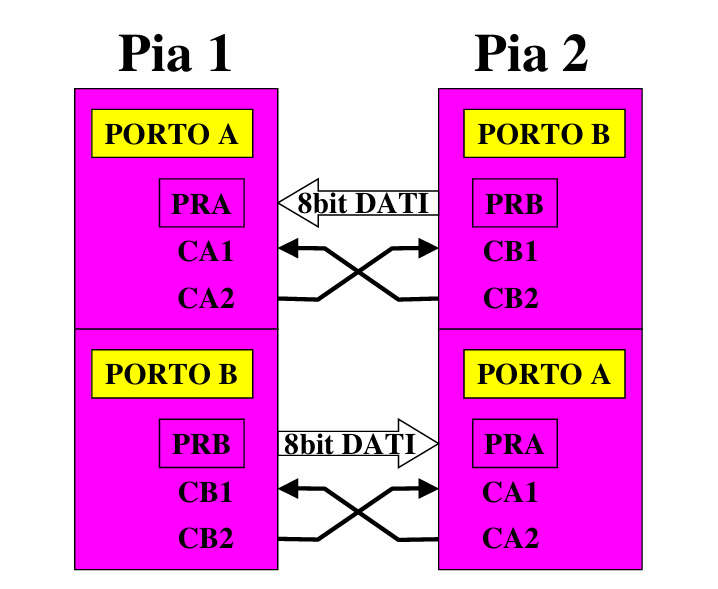
\includegraphics[width=0.75\textwidth]{img/PIA_fd.png}
    \caption{Configurazione Full Duplex}\label{img:PIA_FD}
\end{figure}

Le routine dedicate alla configurazione dei porti A e B sono uguali a quelle viste nell'esercizio 2 di questa sezione (\ref{par:es_1_2}).
La routine dedicata alla configurazione del terminale consta di una sola istruzione e ritorna:

\begin{lstlisting}
    DVTER	MOVE.B	#$3f,TERC	;seleziona indirizzo stato/controllo
	RTS		
\end{lstlisting}

In pratica viene soltanto scritto il bye 00111111 nel registro di controllo/stato del terminale, il cui significato è chiarito dall'immagine \ref{img:terminal_cfg}.

\begin{figure}[!ht]
    \centering
    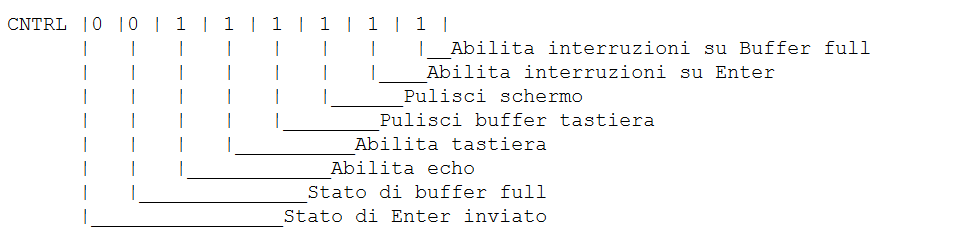
\includegraphics[width=0.5\textwidth]{img/terminal_ctrl.png}
    \caption{Configurazione registro controllo/stato del terminale}
    \label{img:terminal_cfg}
\end{figure}

Dopodichè, il main entra in un ciclo idle in cui attende le interruzioni (dopo averle abilitate sul registro di stato).
Vediamo nel dettaglio la ISR per la gestione dato proveniente dalla tastiera di TERMINAL e spedito, per tramite del PIA porto B, all'altro sistema.
ISR associata all'interrupt di liv. 1, \#vect 25 mappato a \$64 della ROM con ISR a \$8500. 

\begin{lstlisting}
    ORG	$8500		ricevi da tastiera
    INT1	MOVE.L	A0,-(A7)		;push di A0,A1,A2,D0,D1 in stack supervisor
        MOVE.L	A1,-(A7)
        MOVE.L	A2,-(A7)
        MOVE.L	D0,-(A7)
        MOVE.L	D1,-(A7)
        MOVEA.L	#TERD,A0
        MOVEA.L	#PIADB,A1
        MOVEA.L	#PIACB,A2
    
    INPUT	MOVE.B	(A0),D0			;acquisisci dato da terminal
    
    *trasferisci il carattere letto alla PIA-B con handshaking
            MOVE.B  (A1),D1         ;lettura fittizia 
            MOVE.B  D0,(A1)         ;Dato su bus di PIA porto B: dopo la scrittura di PRB, CB2 si abbassa
    *								;cio fa abbassare CA1 sulla porta gemella dell'altro sistema generando 
    *								;un'interruzione che coincide con il segnale DATA READY
        
    ciclo2	MOVE.B	(A2),D1			;In attesa di DATA ACKNOWLEDGE
        ANDI.B	#$80,D1				;aspetta che CRB7 divenga 1
        BEQ	ciclo2
                
    *fine trasferimento e handshaking
        
        CMP.B   	#13,D0		;Se il carattere ricevuto e' ENTER	
        BNE     	INPUT		;termina altrimenti prossimo carattere
        ORI.B	#$1C,TERC		;riabilita tastiera ,pulisce buffer e video
        MOVE.L 	(A7)+,D1		;ripristino di D0,D1,A2,A1,A0
        MOVE.L	(A7)+,D0
        MOVE.L	(A7)+,A2
        MOVE.L	(A7)+,A1
        MOVE.L	(A7)+,A0
        RTE
\end{lstlisting}

In questo caso è presente per forza di cose un ciclo improduttivo (ciclo2) perchè bisogna procedere sequenzialmente al set di istruzioni successivo che prevede un salto a INPUT se il carattere ricevuto non è quello finale (ENTER). Dopodichè resetta il terminale riabilitando tastiera e pulendo buffer e video scrivendo nel registro di controllo in accordo a quanto esposto nella figura \ref{img:terminal_cfg}, e ritorna.

Procediamo vedendo la ISR per il \textit{buffer full}: praticamente è identica a quella per l'acquisizione del messaggio in seguito a ENTER, ma in questo caso vengono inviati tutti e 256 i caratteri conservati nel buffer del terminale.
ISR a \$8600 associata all'interrupt di livello 2 \#vect (24+2) => mappato a 4*26 = 104 = \$68.

\begin{lstlisting}
    ORG	$8600		
    INT2	MOVE.L	A0,-(A7)		;push di A0,A1,A2,D0,D1 in stack supervisore
        MOVE.L	A1,-(A7)
        MOVE.L	A2,-(A7)
        MOVE.L	D0,-(A7)
        MOVE.L	D1,-(A7)
        MOVE.L	D2,-(A7)
        MOVEA.L	#TERD,A0
        MOVEA.L	#PIADB,A1
        MOVEA.L	#PIACB,A2
        MOVE.B	#255,D2		;#caratteri da trasferire
        
    SWAP	MOVE.B	(A0),D0			;acquisisci dato da terminal
    
    *trasferisci il carattere letto alla PIA-B con handshaking
        MOVE.B  (A1),D1         ;lettura fittizia => serve per azzerare CRB7 dopo il primo carattere, altrimenti resta settato con l'ack
        MOVE.B  D0,(A1)         ;Dato su bus di PIA porto B: dopo la scrittura di PRB, CB2 si abbassa
    *							;cio fa abbassare CA1 sulla porta gemella dell'altro sistema generando 
    *							;un'interruzione che coincide con il segnale DATA READY
        
        
    ciclo3	MOVE.B	(A2),D1		;In attesa di DATA ACKNOWLEDGE
        ANDI.B	#$80,D1		;aspetta che CRB7 divenga 1
        BEQ	ciclo3
                
    *fine trasferimento e handshaking
            
        DBRA    	D2,SWAP	;contatore di bit inviati	
        ORI.B	#$1C,TERC	;riabilita tastiera ,pulisce buffer e video
        MOVE.L	(A7)+,D2	;ripristino di D0,D1,A2,A1,A0
        MOVE.L 	(A7)+,D1
        MOVE.L	(A7)+,D0
        MOVE.L	(A7)+,A2
        MOVE.L  	(A7)+,A1
        MOVE.L  	(A7)+,A0
        RTE
\end{lstlisting}

L'ultima interruzione è quella che scatena il porto A in seguito alla ricezione di un carattere. 

\begin{lstlisting}
    ORG $8700		

    INT3    	ANDI.B		#%11101001,TERC	;disabilita: tastiera,cancella video,interruzioni su enter		 
        MOVE.L  A1,-(A7)		;salvataggio registri
        MOVE.L  A0,-(A7)
        MOVE.L  D0,-(A7)
    
        MOVEA.L  #TERD,A0	;inizializzazione indirizzi device
        MOVEA.L  #PIADA,A1
        
        MOVE.B 	(A1),(A0)	;acquisisce il carattere e lo trasferisce a Terminal
    *						;la lettura da PRA fa abbassare CRA7 e CA2 => nell'altro sistema si abbassa CB1
    *						;cio corrisponde all'attivazione di CRB7 che funge da DATA ACKNOWLEDGE
        
        MOVE.L  (A7)+,D0		;ripristino registri 
        MOVE.L  (A7)+,A0
        MOVE.L  (A7)+,A1
        
        ORI.B	#$12,TERC	;riabilita tastiera e interruzioni su enter 
        RTE
    
    
        END	BEGIN
\end{lstlisting}

